\documentclass{beamer}
\usetheme{Singapore}
%\usetheme{Copenhagen}
\usecolortheme{seahorse}

\usepackage[utf8]{inputenc}

\usepackage{listings, float, graphicx, lipsum, parallel, verbatim, mathtools, amssymb, hyperref}

\title{cDCGAN}
\subtitle{conditional Deep Convolutional Generative Adversarial Networks}
\author{Edoardo De Matteis}
\date{}

\institute[La Sapienza University of Rome]

\begin{document}

\frame{\titlepage}

% * GAN.
\section{GAN}

\begin{frame}{Generative adversarial networks}
    The idea behind generative models is to learn a distribution from training data and generate new samples from it.
    GANs do it setting up a zero-sum game between a \textbf{discriminator} and a \textbf{generator}.
\end{frame}

\begin{frame}
    \centering
    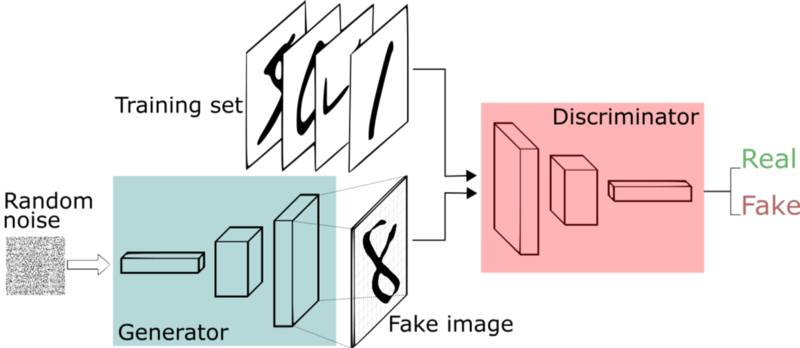
\includegraphics[scale=0.35]{images/gan-scheme-rand.png}
\end{frame}

% * DCGAN.
\section{DCGAN}
\begin{frame}{DCGAN}
    GANs where first introduced based only on FC layers, it came natural to extend them with convolutions when dealing with images.

    To make them more stable to train we can constraint their architectural topology.
\end{frame}

\begin{frame}{Architectural guidelines}
    \begin{itemize}
        \item \textit{All-convolutional net} i.e. replace deterministic spatial pooling with strided convolutions, allowing the network to learn its own spatial downsampling/upsampling.
        \item Eliminate fully connected layers on top of CNNs in favor of deeper architectures.
    \end{itemize}
\end{frame}

\begin{frame}
    \begin{itemize}
        \item Use of batch normalization in both the generator and discriminator, yet the first could be made unstable.
        \item Use ReLU activation in generator for all layers except for the output, which uses Tanh, and use LeakyReLU activation in the discriminator for all layers.
    \end{itemize}
\end{frame}

\begin{frame}
    \centering
    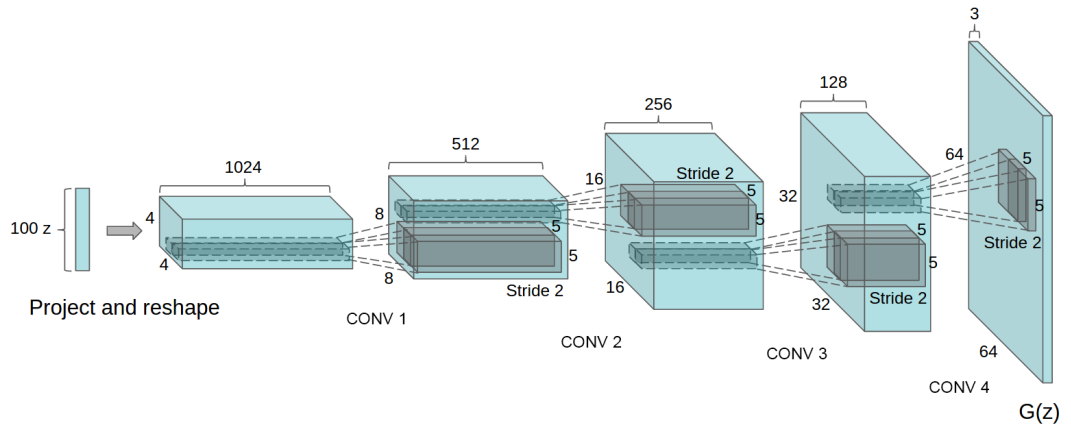
\includegraphics[scale=0.37]{images/dcgan-scheme.png}
\end{frame}

\begin{frame}{Results}
    It is hard in general to train GANs, after a few epochs with a small learning rate the generator learns well general features, yet it still far from realism.
\end{frame}

\begin{frame}{LSUN}
    \centering
    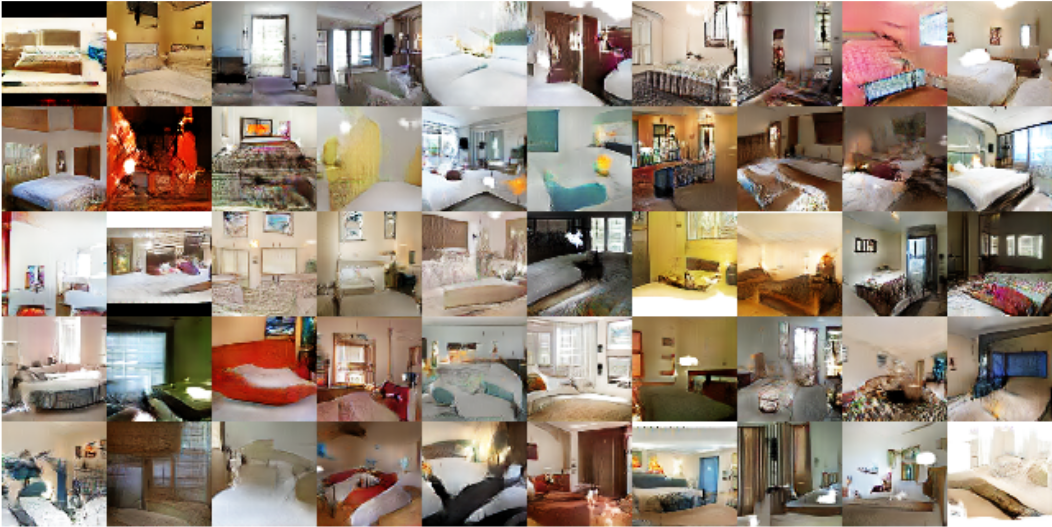
\includegraphics[scale=0.35]{images/dcgan-results.png}
\end{frame}

% * CGAN
\section{cGAN}
\begin{frame}{cGAN}
    One issue with GANs is that we cannot choose which output we get, hower by conditioning the model on additional information is possible to direct data generation.
\end{frame}

\begin{frame}
    \centering
    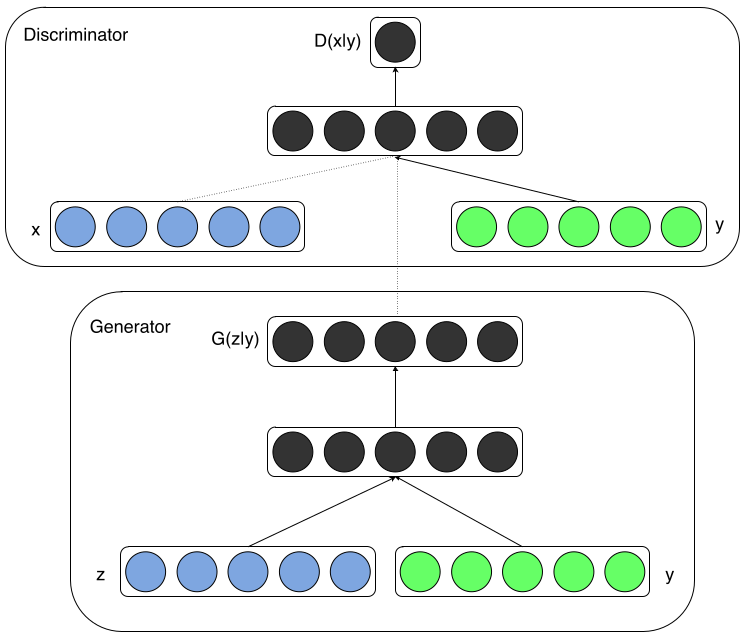
\includegraphics[scale=0.35]{images/cgan-scheme.png}
\end{frame}

% * cDCGAN.
\section{cDCGAN}
\begin{frame}{cDCGAN}
    Combine the strengths of three models:
    \begin{itemize}
        \item \textit{GAN}: Great generative model.
        \item \textit{DCGAN}: Strong priors on images.
        \item \textit{cGAN}: Conditional model.
    \end{itemize}
\end{frame}

\begin{frame}{Motivations}
    \begin{itemize}
        \item Adding conditional data can have a regularizing effect.
        \item Specialized data enrichment.
        \item Entertainment e.g. \textit{FaceApp}.
        \item Integration with other branches e.g. text to image.
        \item \dots
    \end{itemize}
\end{frame}

\begin{frame}{Dataset}
    \begin{itemize}
        \item MNIST.
        \item FashionMNIST.
        \item CIFAR10.
    \end{itemize}
    Data normalized by z-score and resized to $64 \times 64$ resolution.

    Random samples have dimension 64 and conditioning is directly concatenated as a channel to input vectors.
\end{frame}

\begin{frame}{Discriminator}
    \centering
    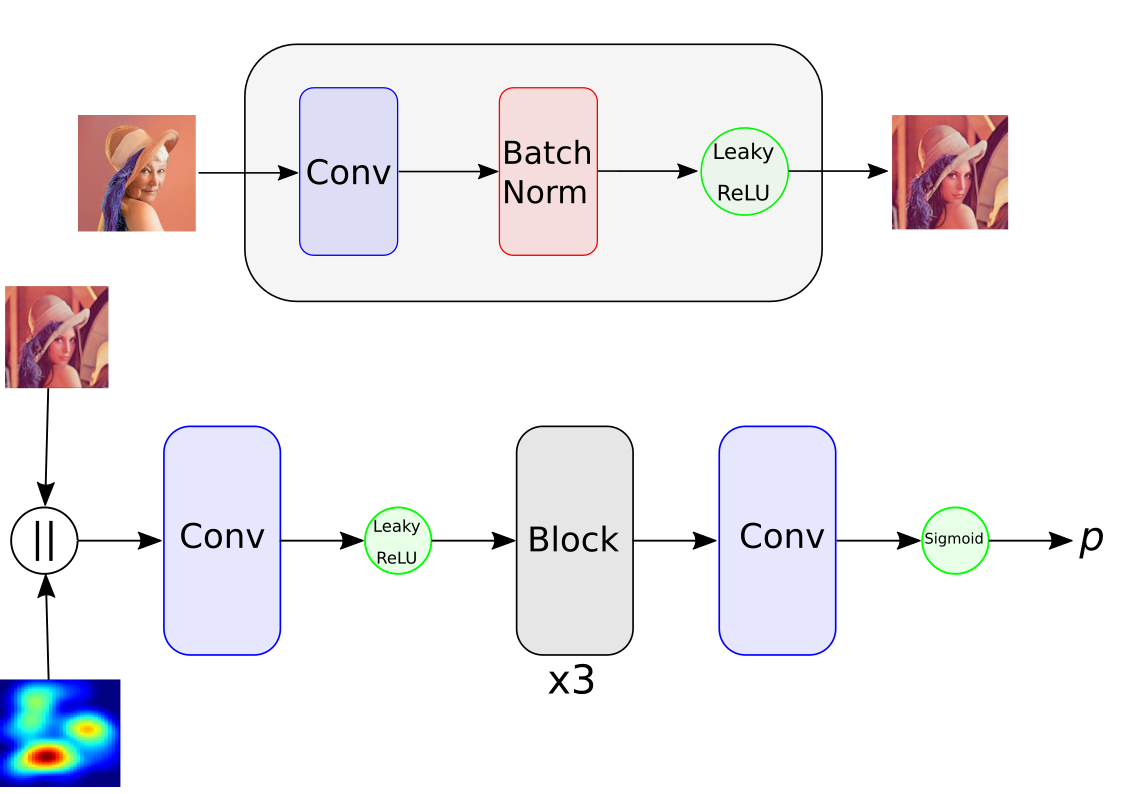
\includegraphics[scale=0.35]{images/discr.png}
\end{frame}

\begin{frame}{Generator}
    \centering
    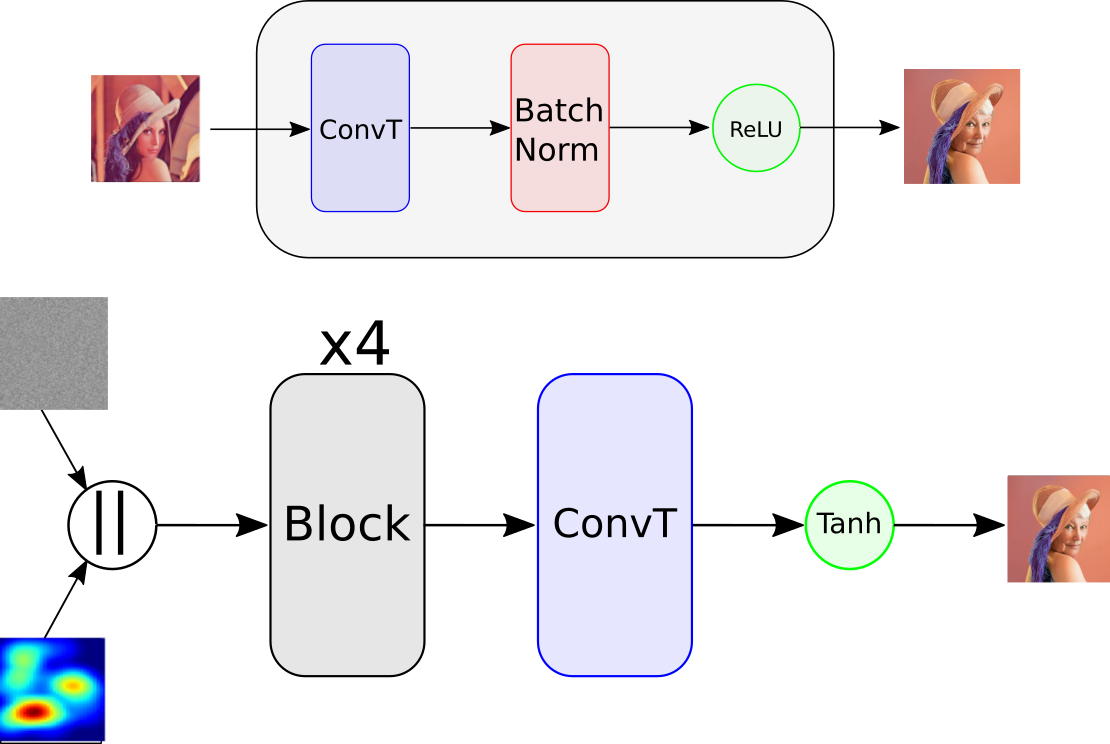
\includegraphics[scale=0.35]{images/gen.png}
\end{frame}

\begin{frame}{Loss}
    \begin{equation}
        \mathcal{L}_{GAN} = \min_\gamma \max_\delta \mathbb{E}_{x \sim p_d} \log D(x) + \mathbb{E}_{z \sim \mathcal{N}} \log (1-D(G(z)))
    \end{equation}
    \begin{equation}
        BCE = -\frac{1}{N} \sum_{i=1}^N y_i \log (f(x_i)) + (1-y_i) \log (1-f(x_i))
    \end{equation}

    We define the ground truth on real and fake data as a vector of ones and zeros respectively.
\end{frame}

\begin{frame}{MNIST}
    \centering
    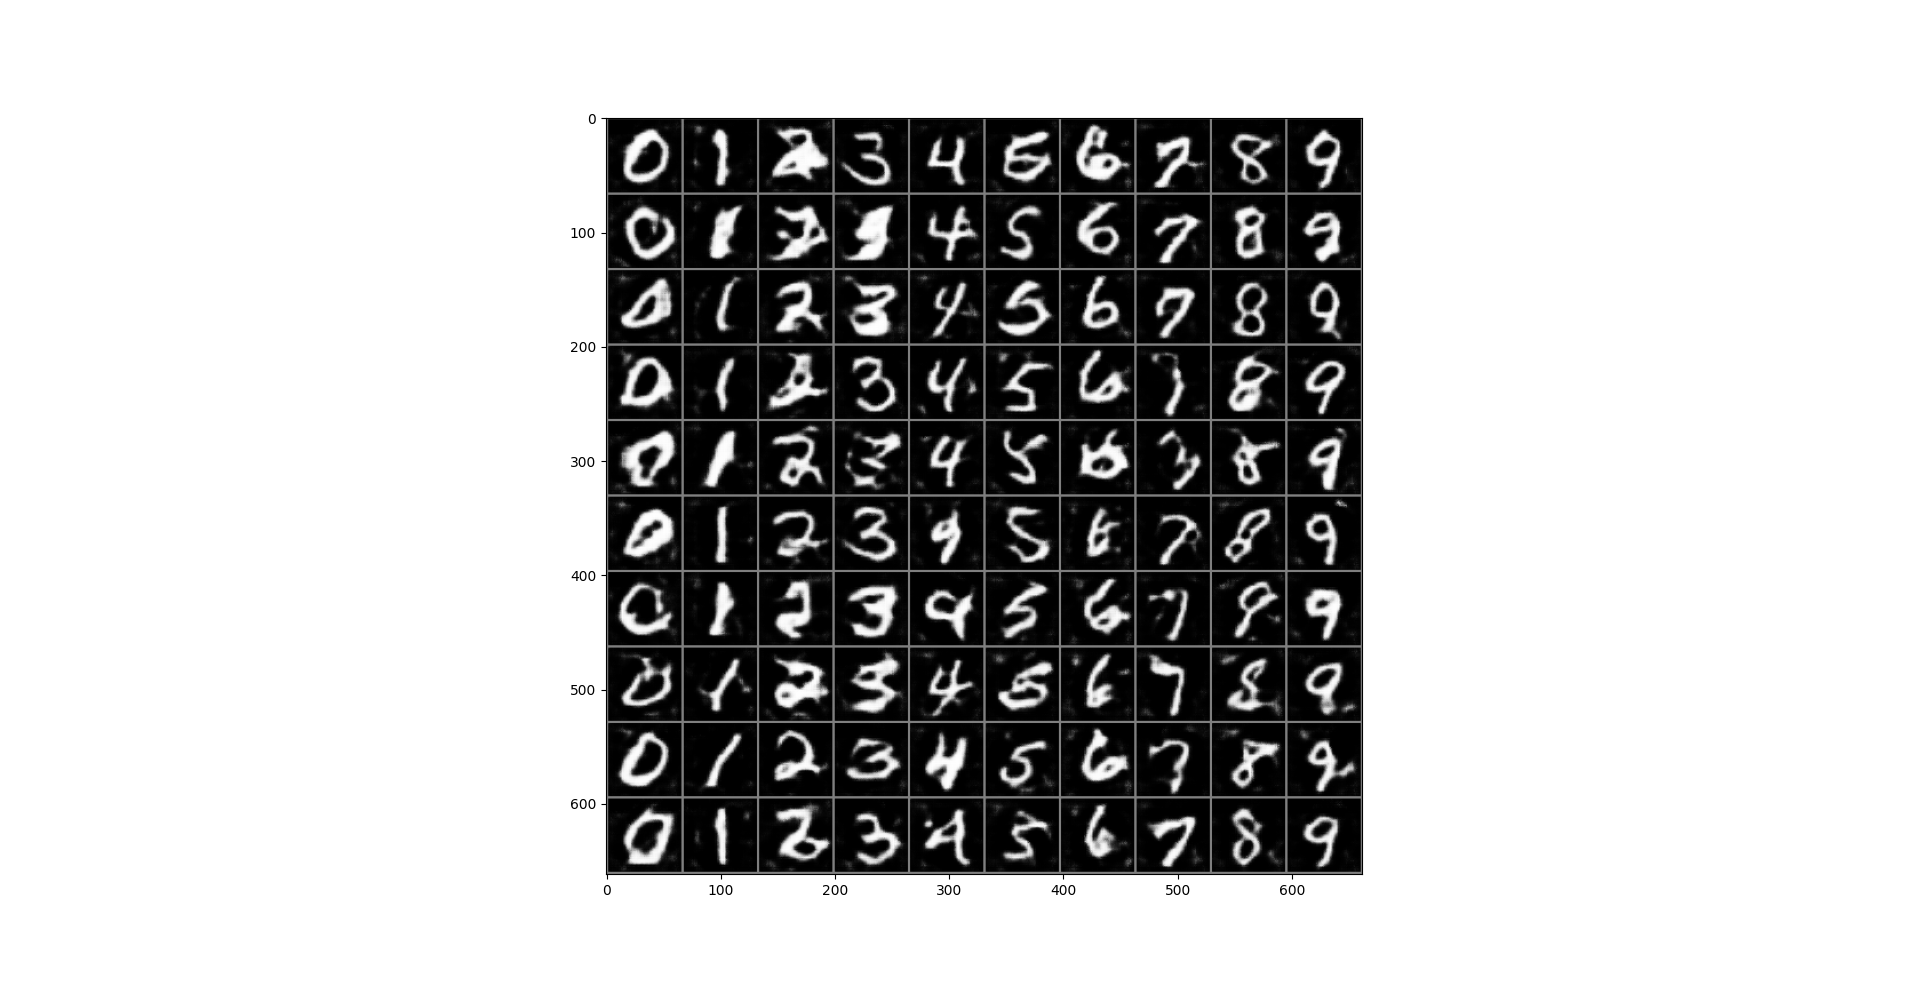
\includegraphics[scale=0.2]{images/mnist.png}
\end{frame}

\begin{frame}{Weighting conditioning}
    \centering
    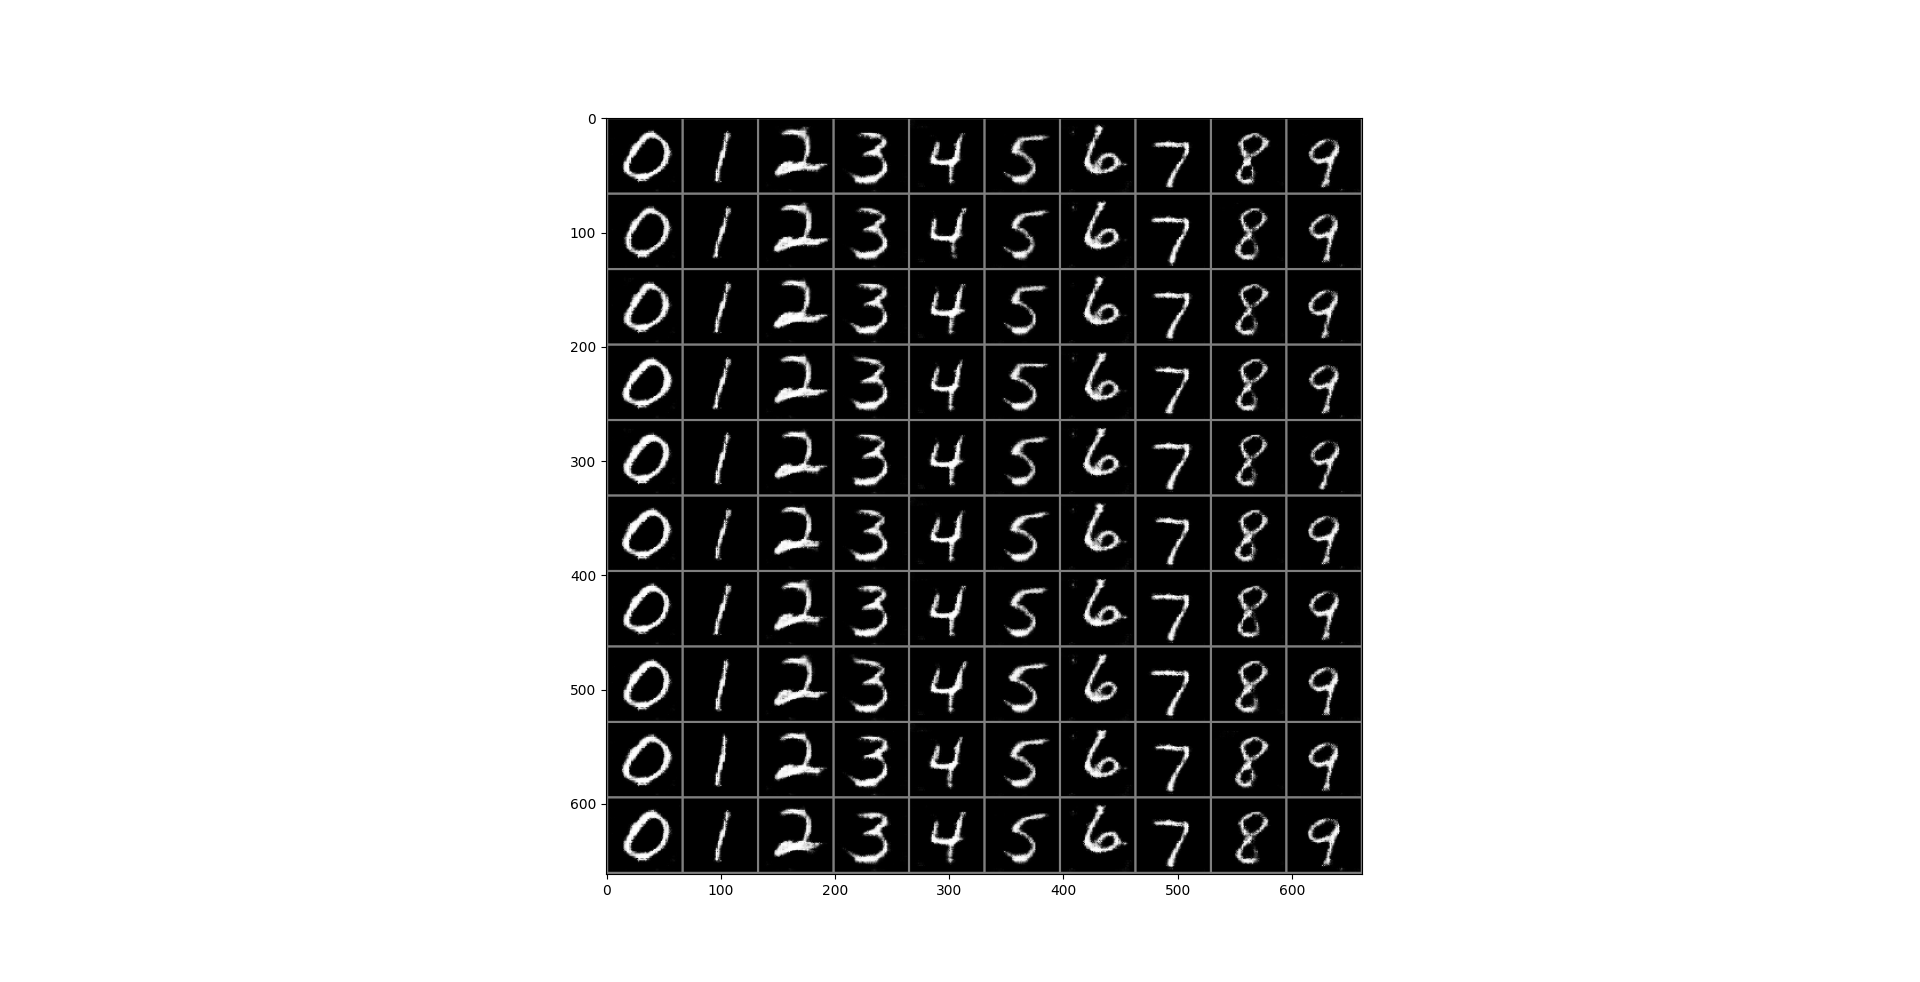
\includegraphics[scale=0.2]{images/mnist-weighted.png}
\end{frame}

\begin{frame}{FashionMNIST}
    \centering
    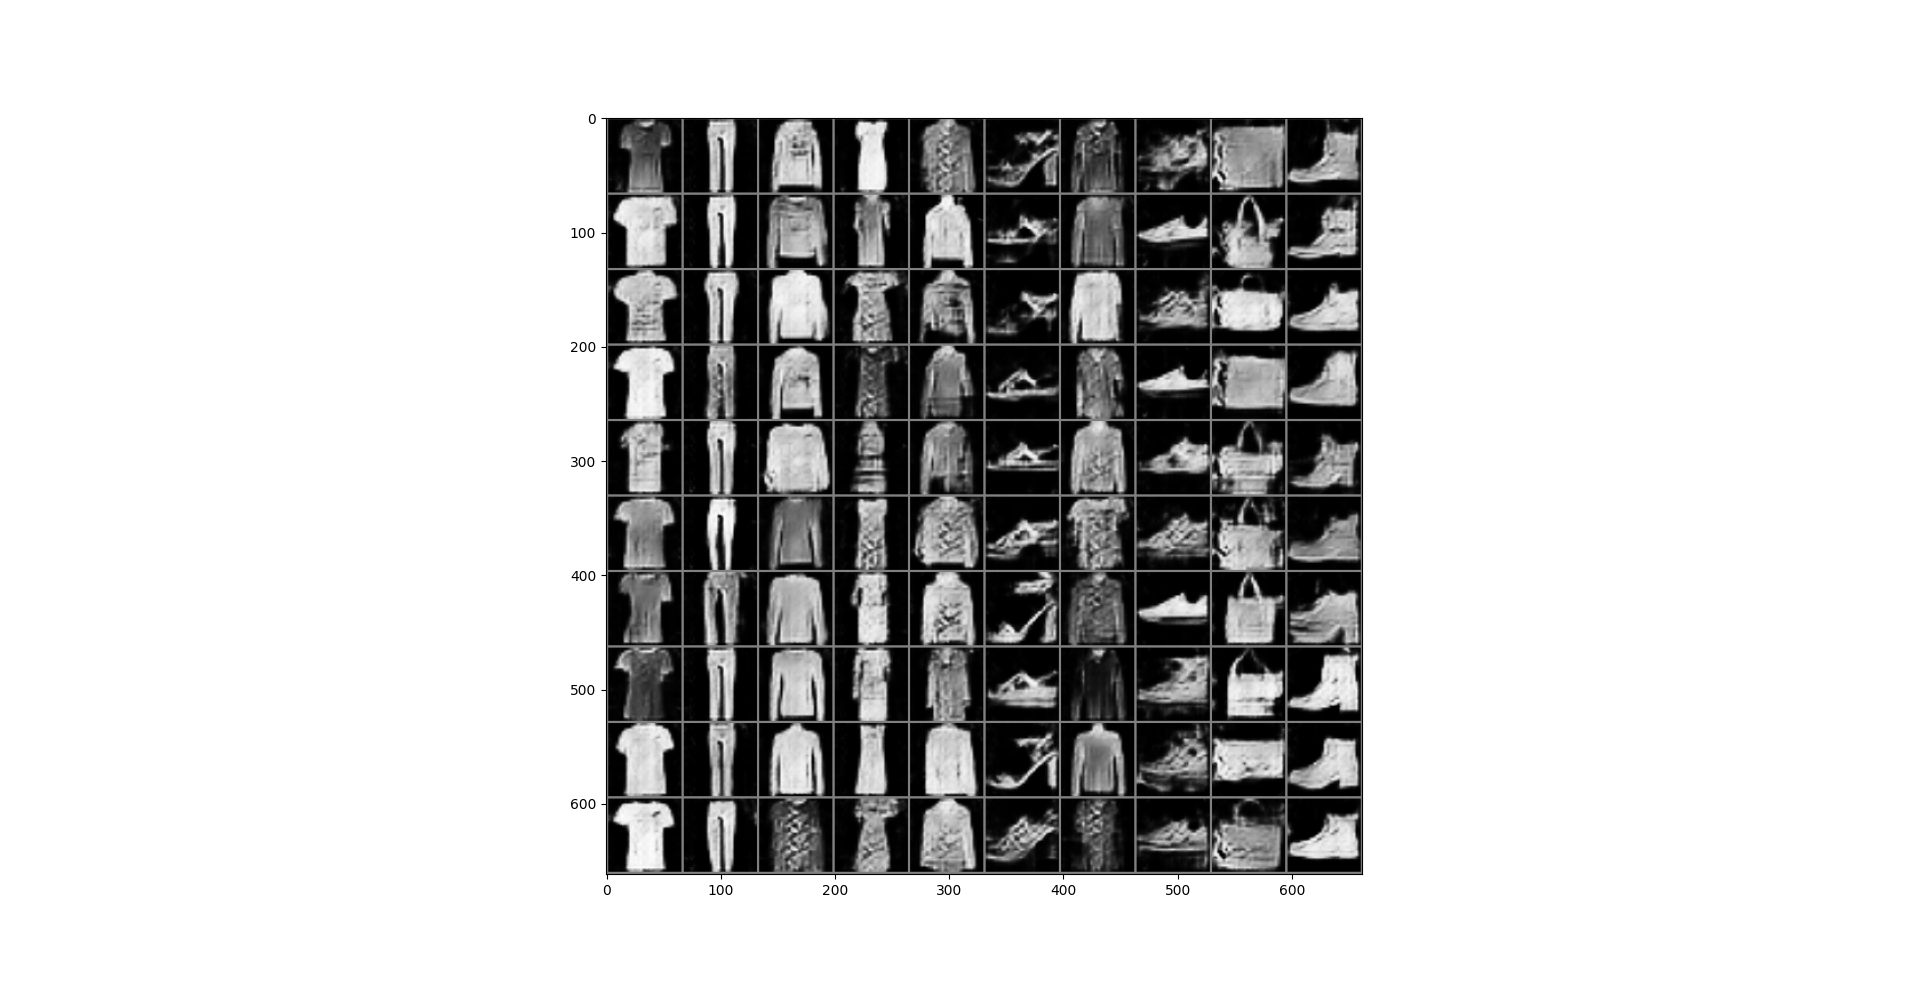
\includegraphics[scale=0.2]{images/fashion.png}
\end{frame}

\begin{frame}{Doing the same\dots}
    \centering
    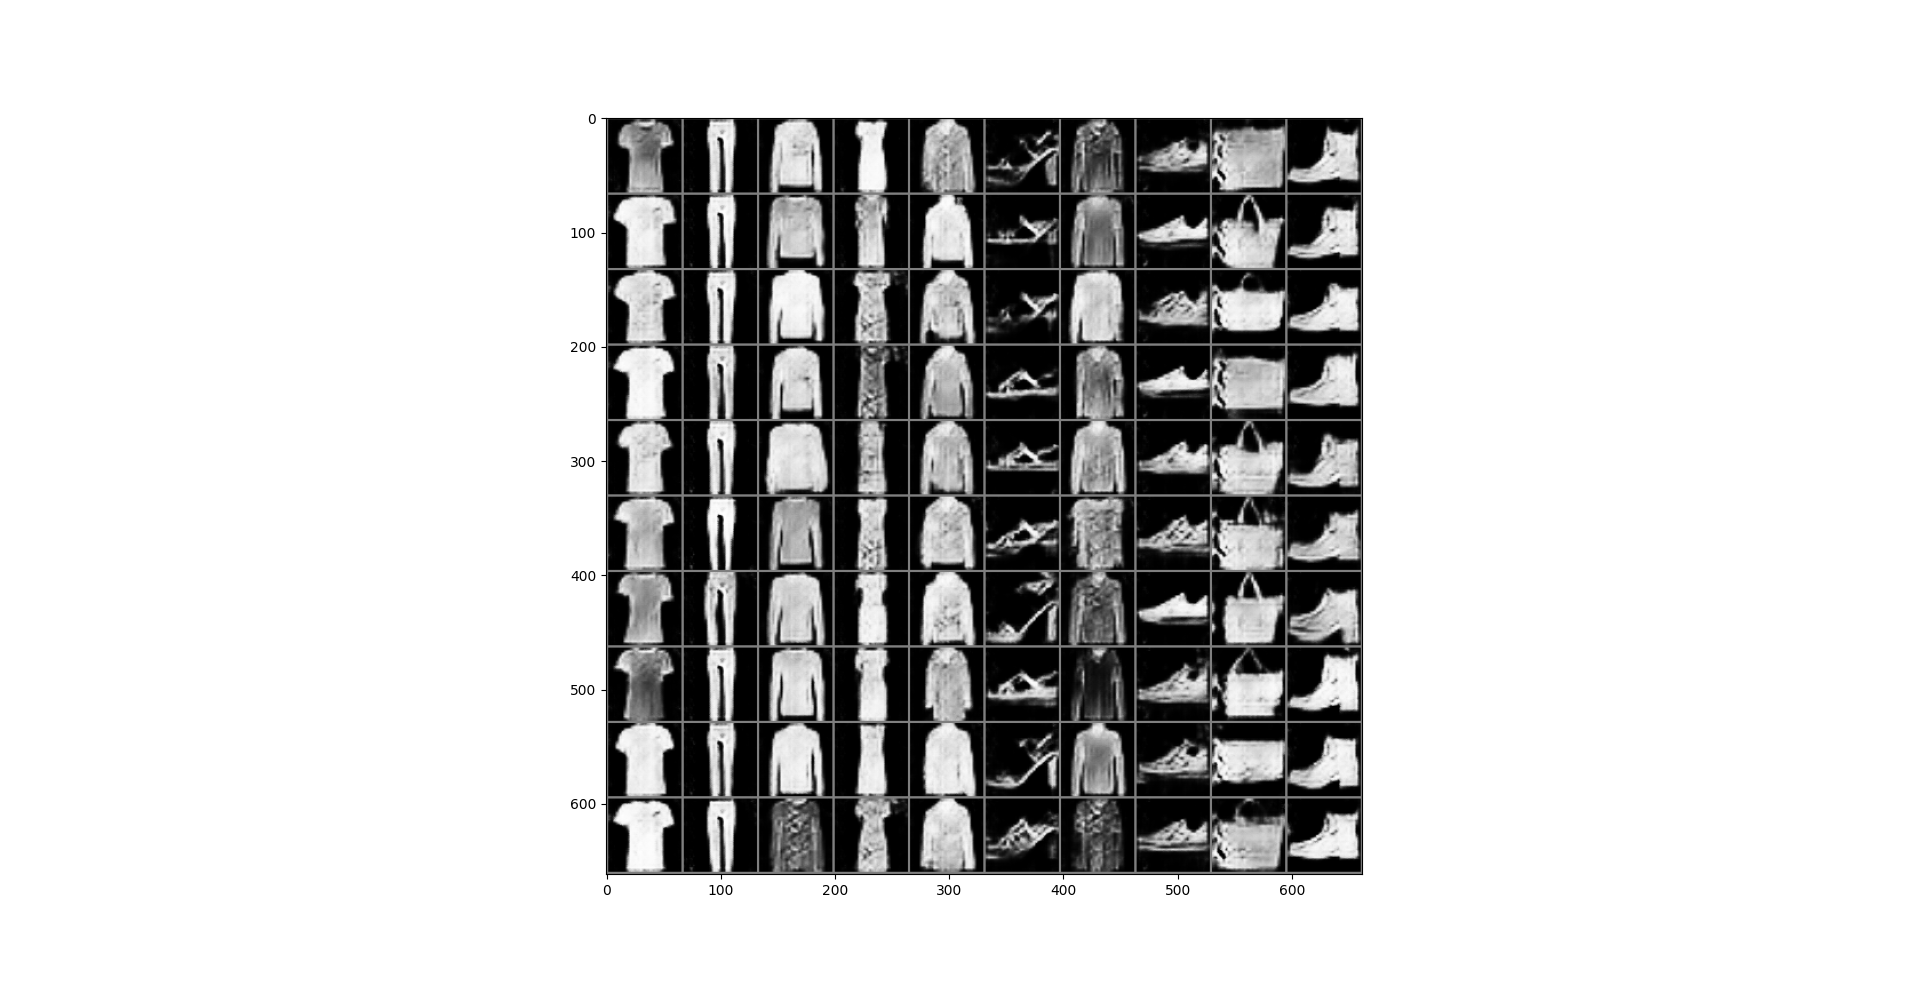
\includegraphics[scale=0.2]{images/fashion-weighted.png}
\end{frame}

\begin{frame}{Multiclass conditioning}
    \centering
    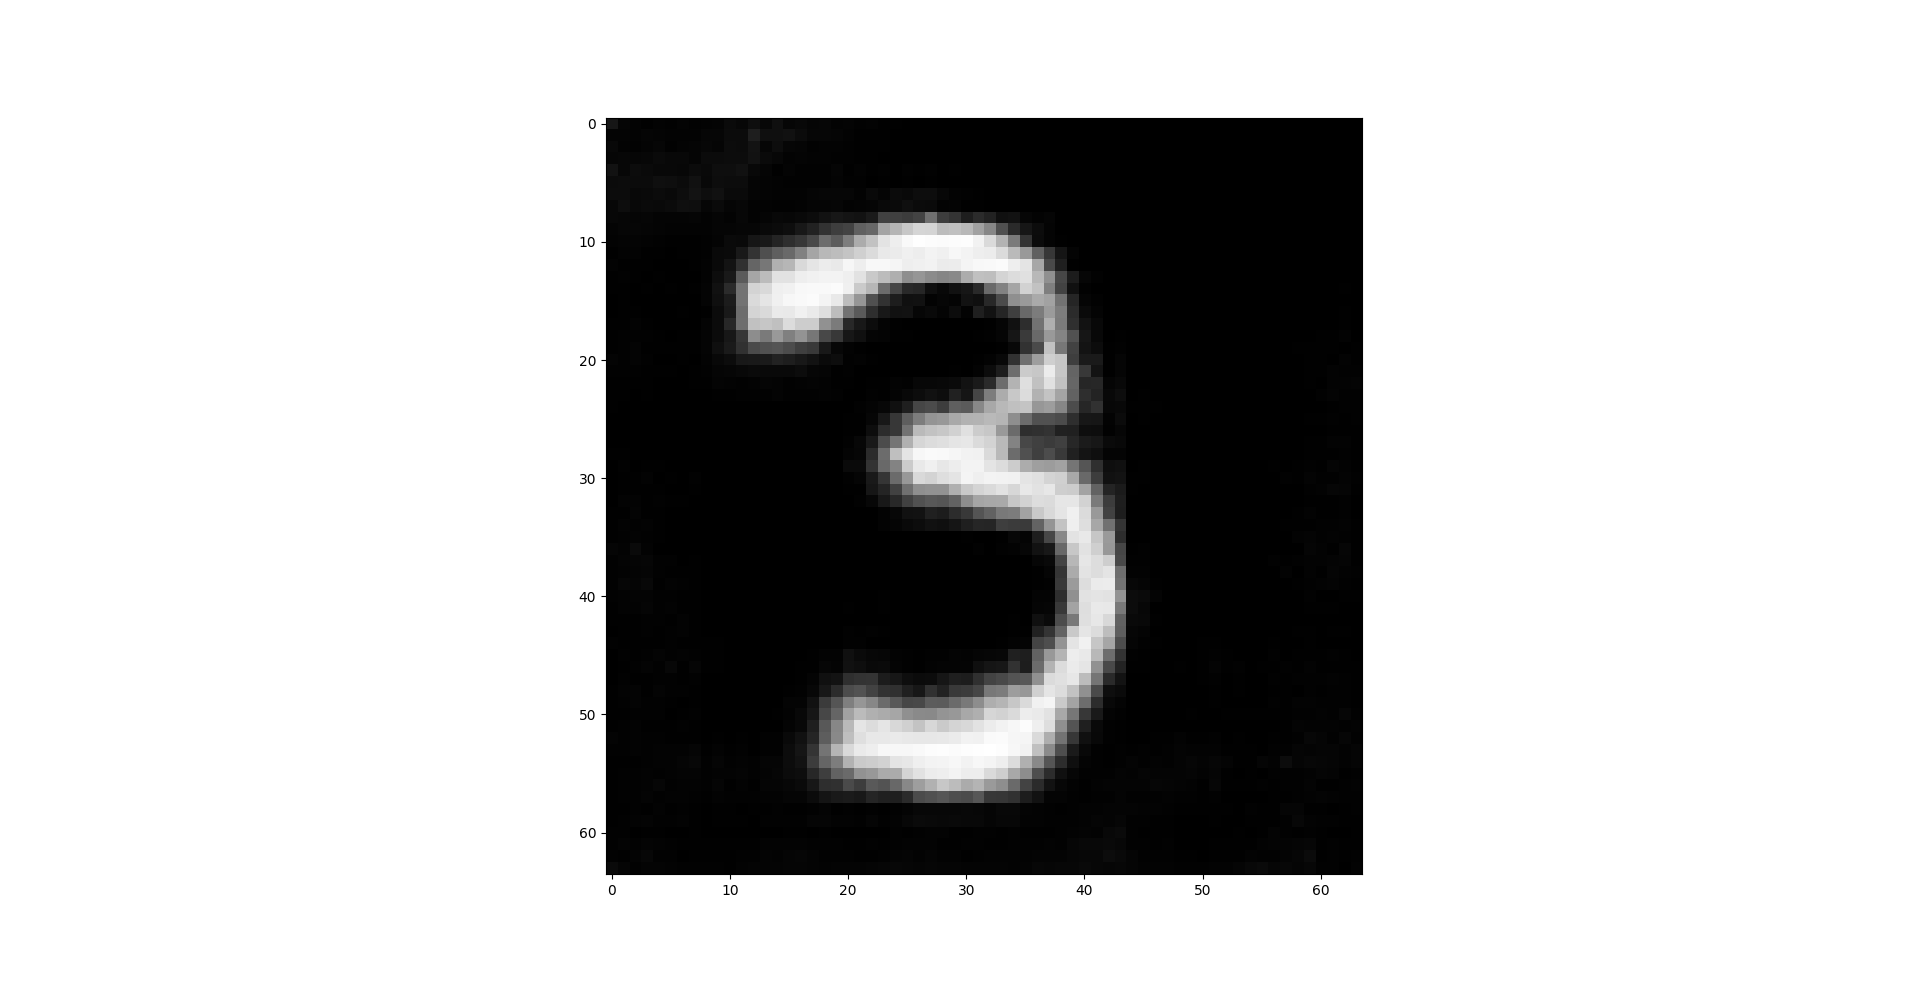
\includegraphics[scale=0.2]{images/gen3.png}
\end{frame}

\begin{frame}
    \centering
    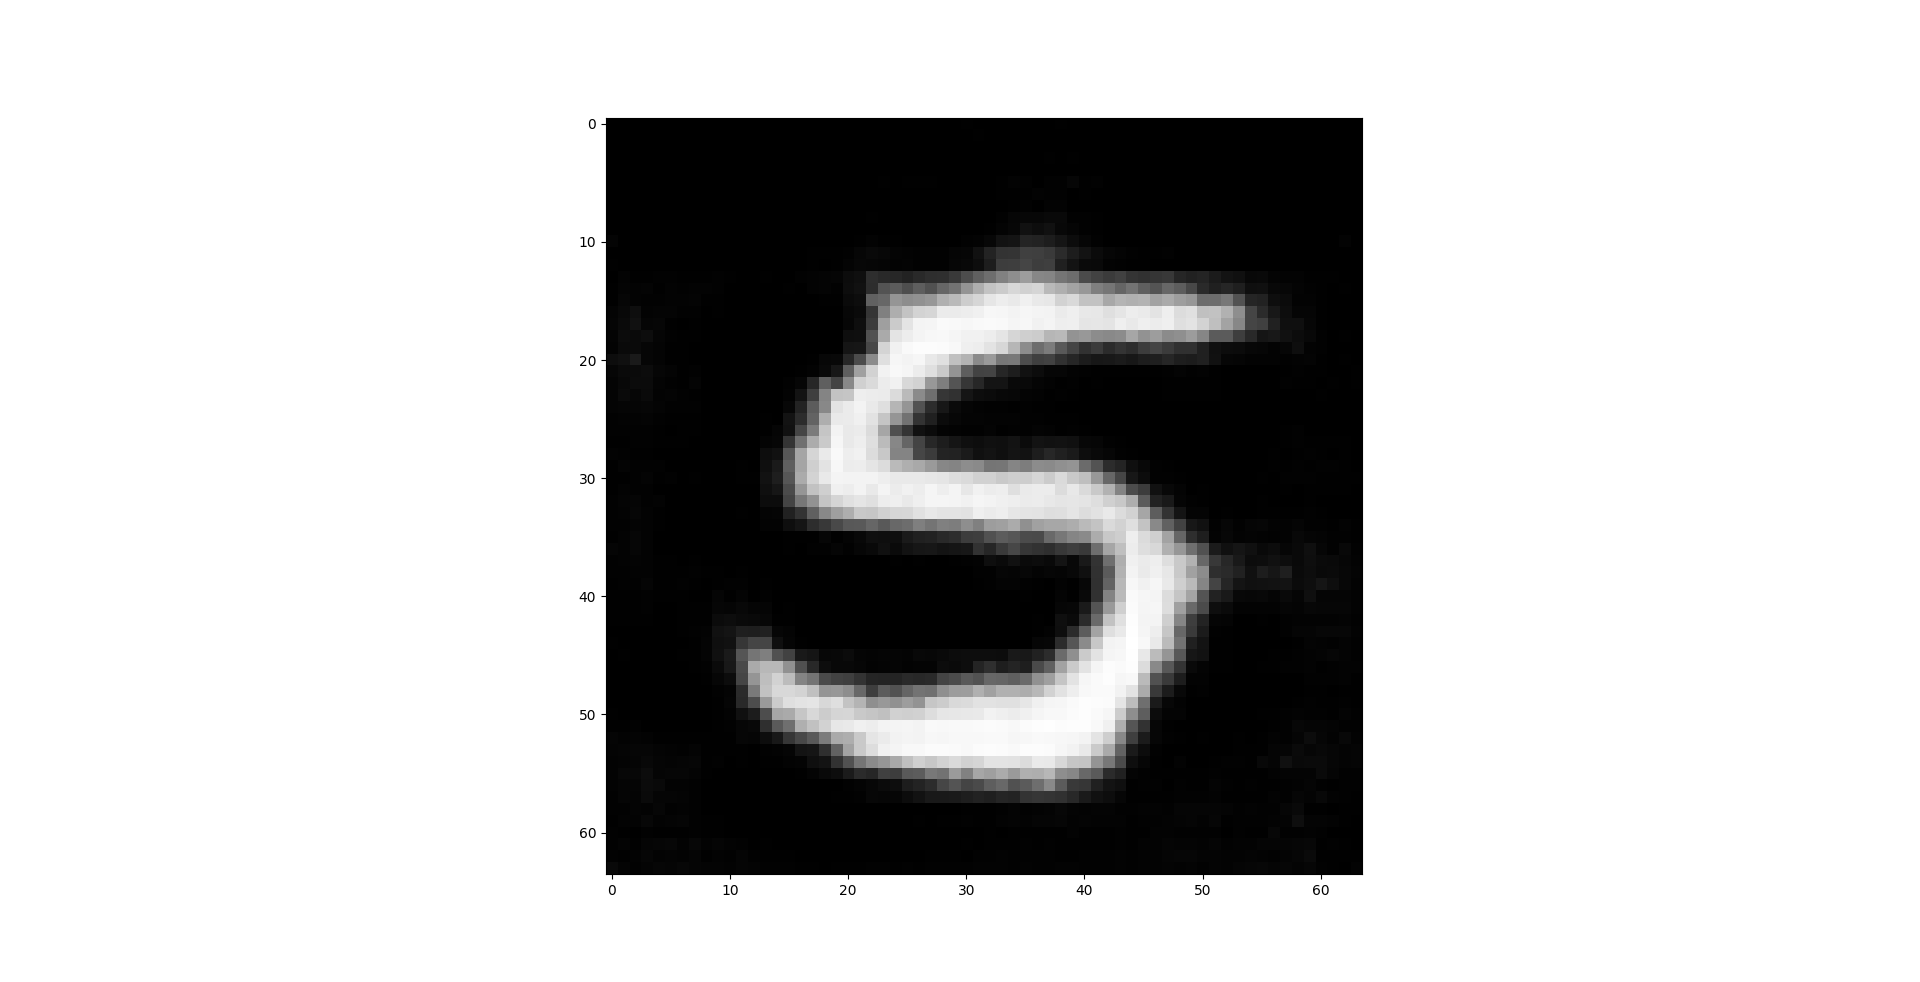
\includegraphics[scale=0.2]{images/gen5.png}
\end{frame}

\begin{frame}
    \centering
    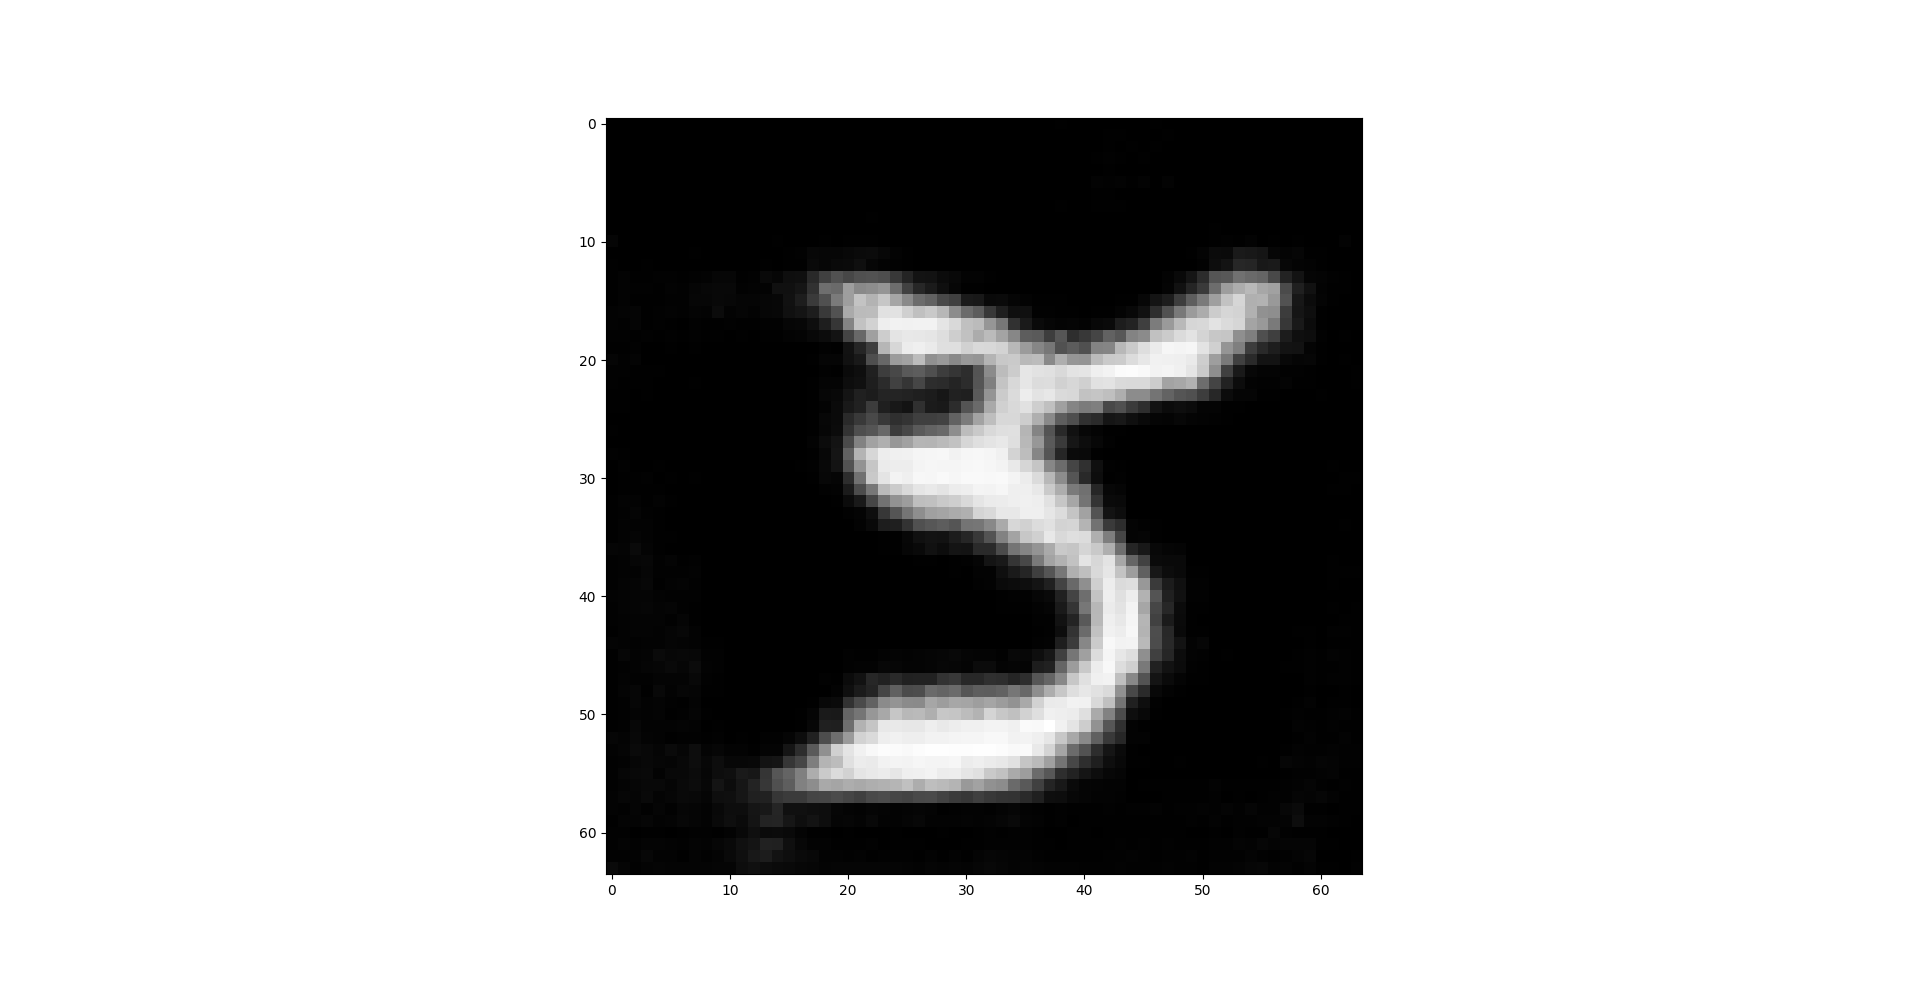
\includegraphics[scale=0.2]{images/gen35.png}
\end{frame}

\begin{frame}{With different weights}
    \centering
    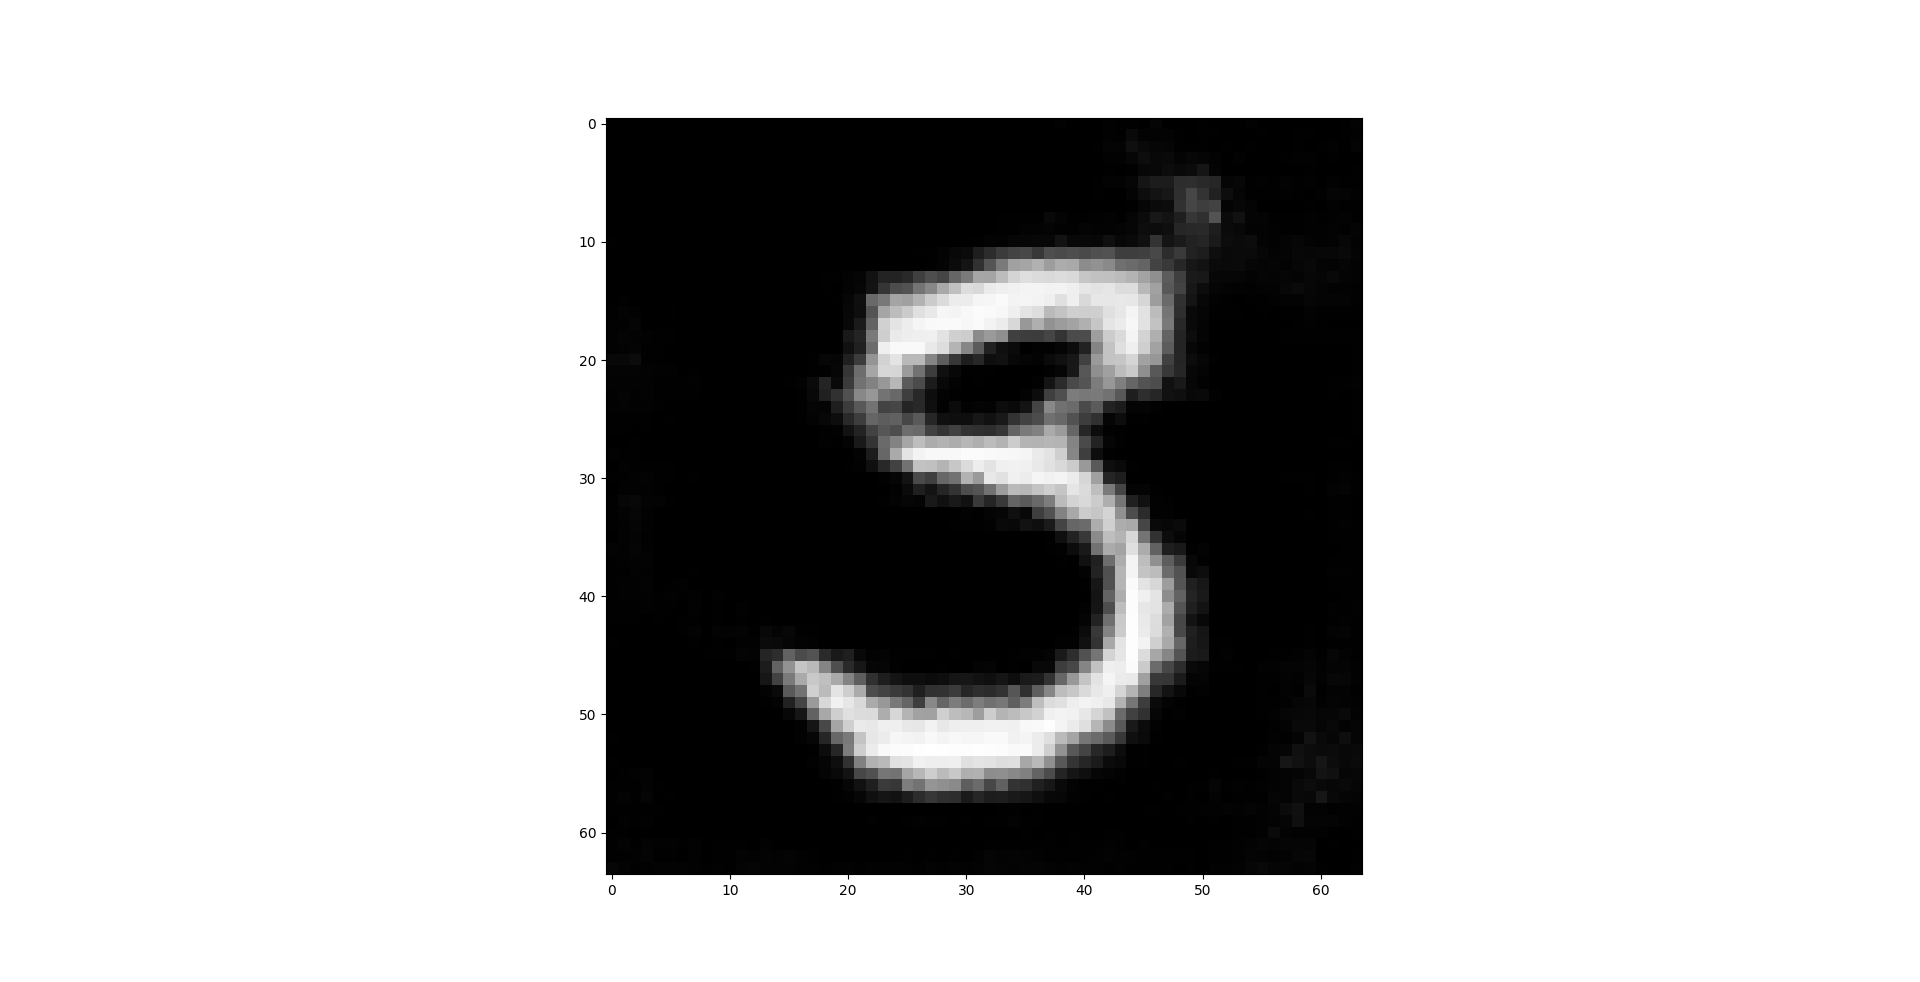
\includegraphics[scale=0.2]{images/gen35with3weighted.png}
\end{frame}

\begin{frame}
    \centering
    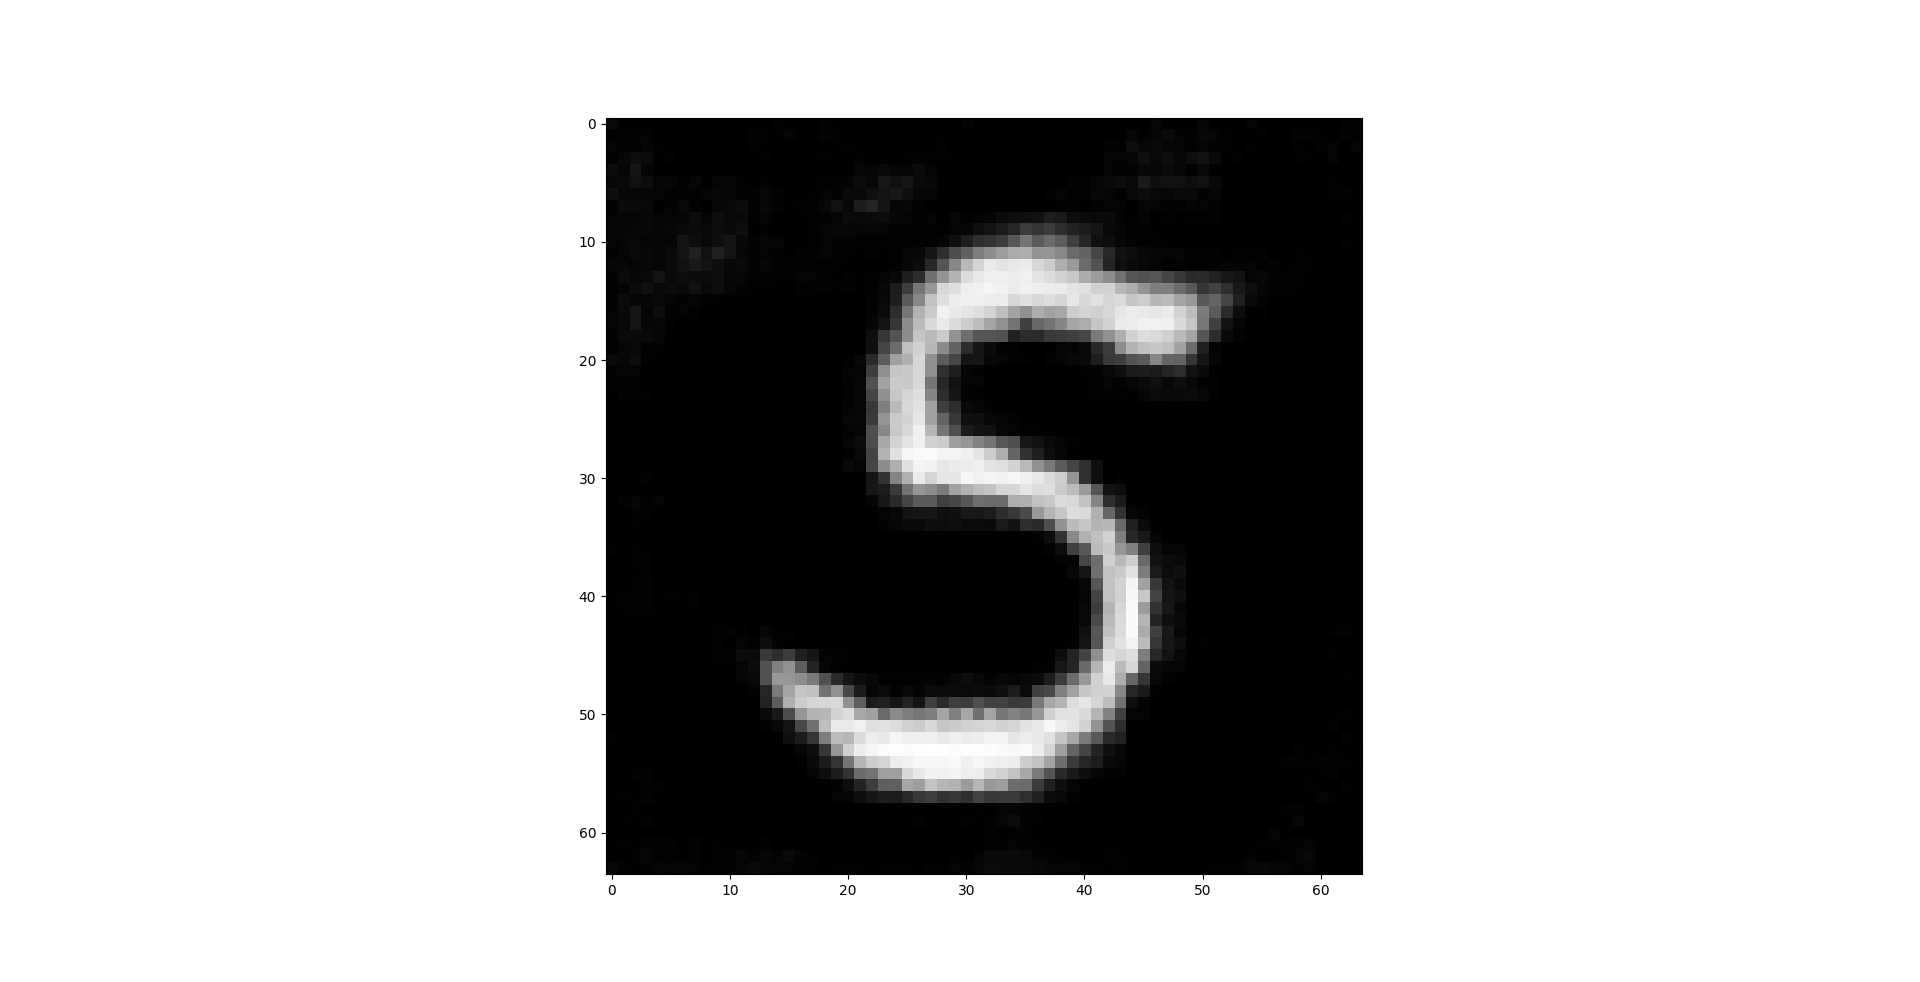
\includegraphics[scale=0.2]{images/gen35with5weighted.png}
\end{frame}

\begin{frame}{The same on FashionMNIST}
    \centering
    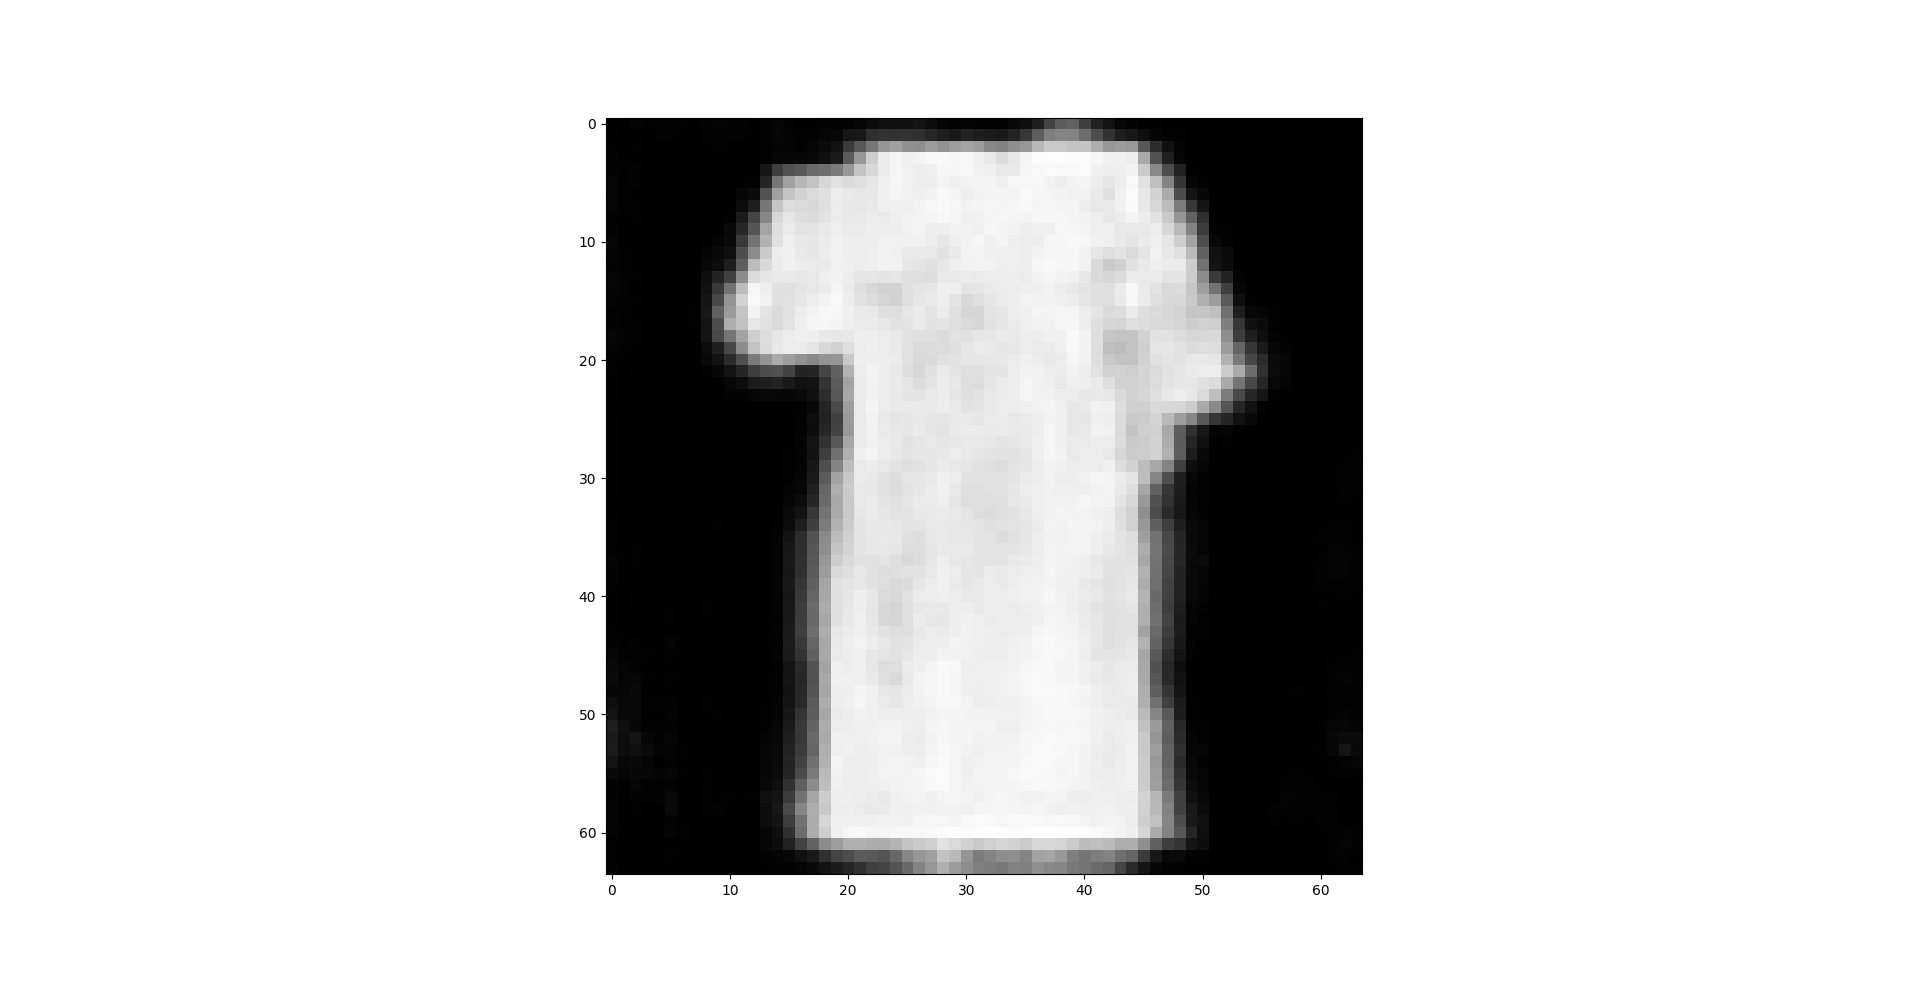
\includegraphics[scale=0.2]{images/shirt.png}
\end{frame}

\begin{frame}
    \centering
    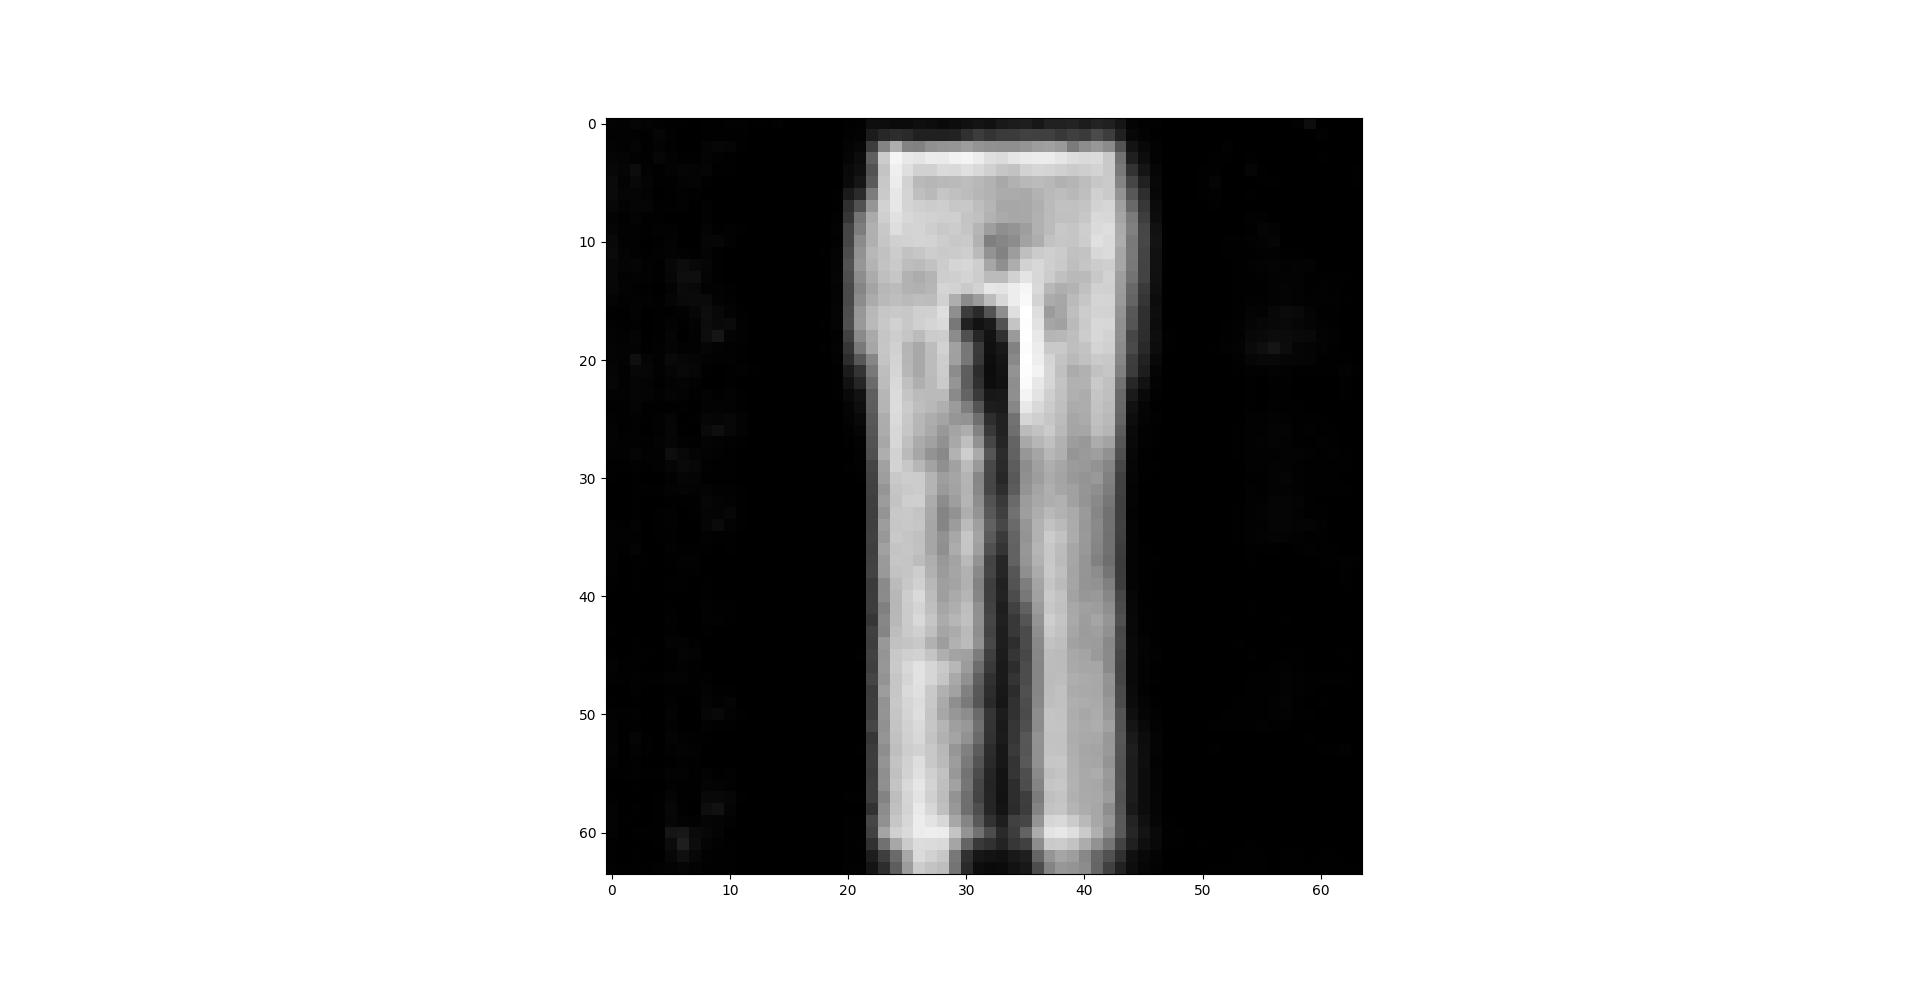
\includegraphics[scale=0.2]{images/pants.png}
\end{frame}

\begin{frame}
    \centering
    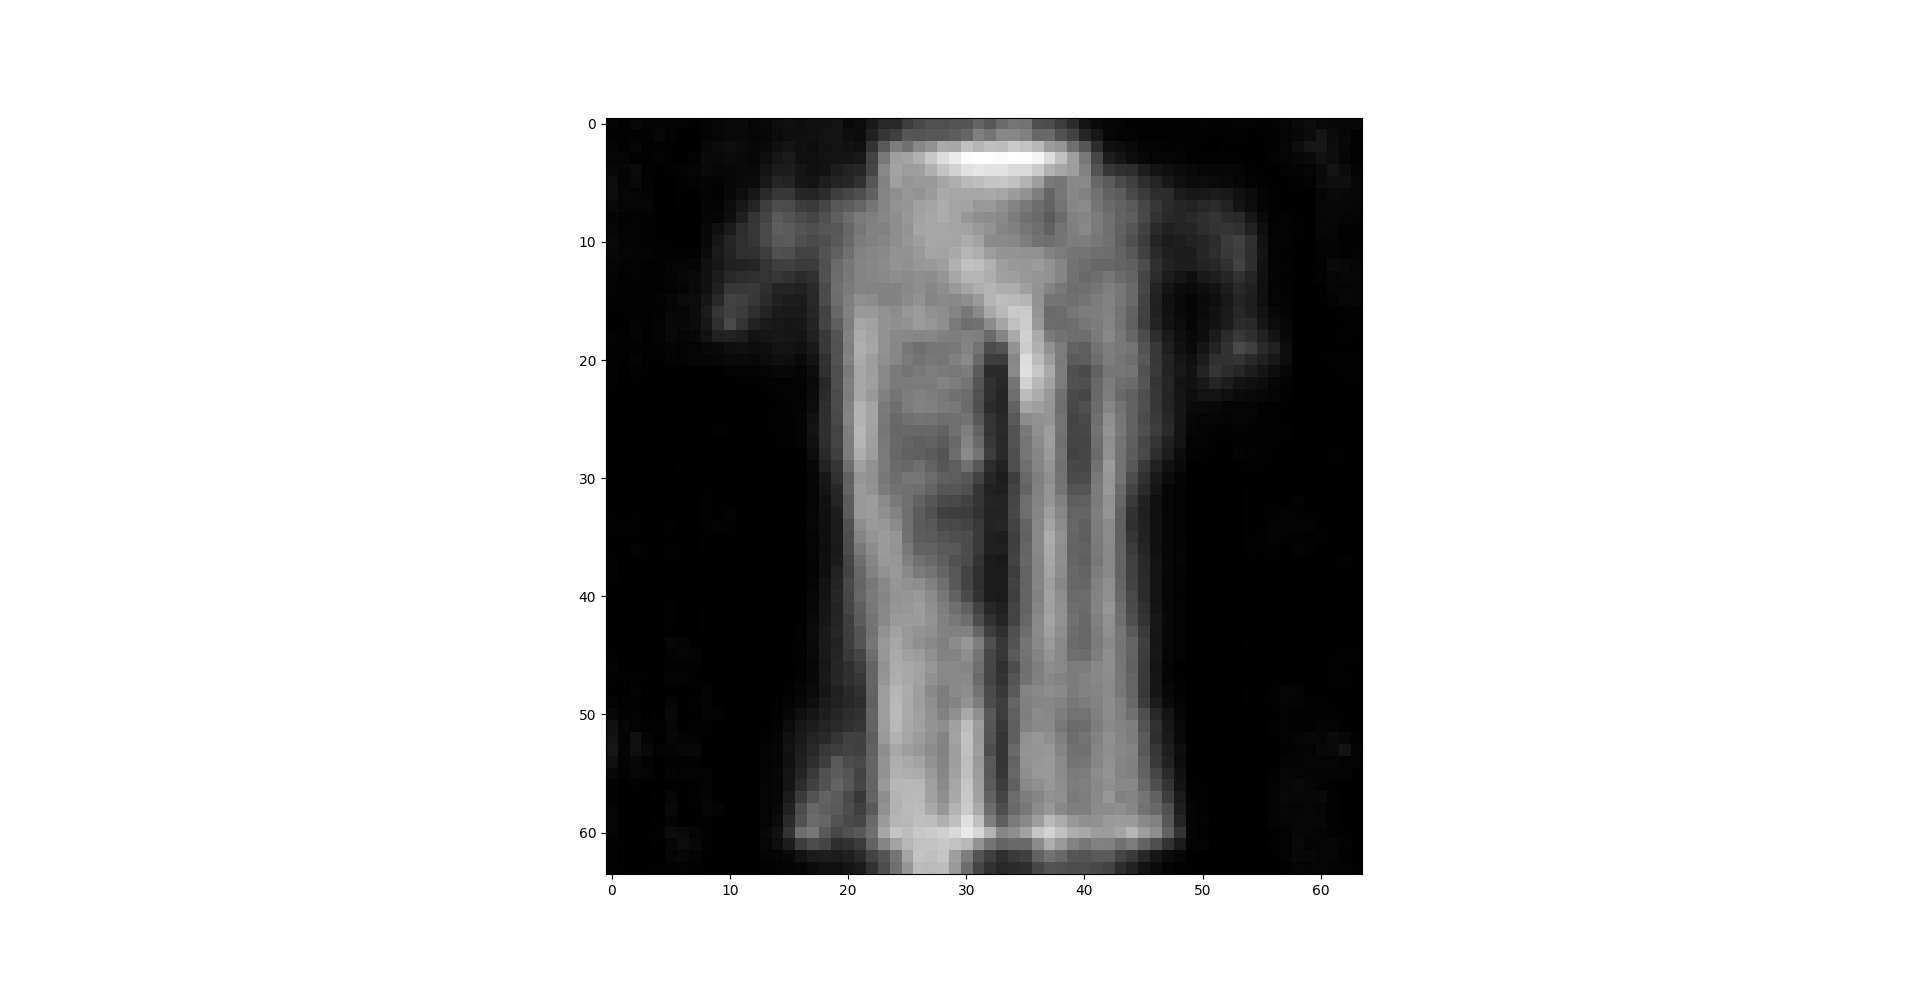
\includegraphics[scale=0.2]{images/shirtpants-weighted.png}
\end{frame}

\begin{frame}
    \centering
    \huge{\textit{Thank you}}
\end{frame}


% * References.
\begin{frame}{References}
    \begin{thebibliography}{}

        \bibitem{dcgan}
        A. Radford, L. Metz, S. Chintala
        \newblock \emph{Unsupervised representation learning with deep convolutional generative adversarial networks}.

        \bibitem{cgan}
        M. Mirza, S. Osindero
        \newblock \emph{Conditional generative adversarial nets}.

    \end{thebibliography}
\end{frame}

\end{document}

